\section{Tests}

Das kontinuierliche Testen und Bewerten aller Einzelkomponenten und Funktionen des Systems ist ein elementarer Entwicklungsbestandteil und teilt den Entwicklungsprozess in unterschiedliche Abschnitte.

Leider hat die aktuell herrschende Covid-19 Pandemie die Erstellung und Durchführung aussagekräftiger Tests erschwert. 

\subsection{Mikrofontest}

Noch vor der eigentlichen Entwicklungsarbeit wurden die zur Verfügung gestellten Einzelkomponenten auf ihre Funktion überprüft. Hierzu wurde der Raspberry Pi mit einem Betriebssystem versehen (Raspberry OS 10) und mit der notwendigen c-Bibliothek versehen BCM 2835 V1.68. Über einfache Jumperkabel wurde jeweils ein zu testendes Mikrofon und ein Abschlussmikrofon an den Raspberry angeschlossen und ein Test durchgeführt. (\autoref{fig:BlockbildMikroTest}).

\begin{figure}[h]
	\begin{center}
		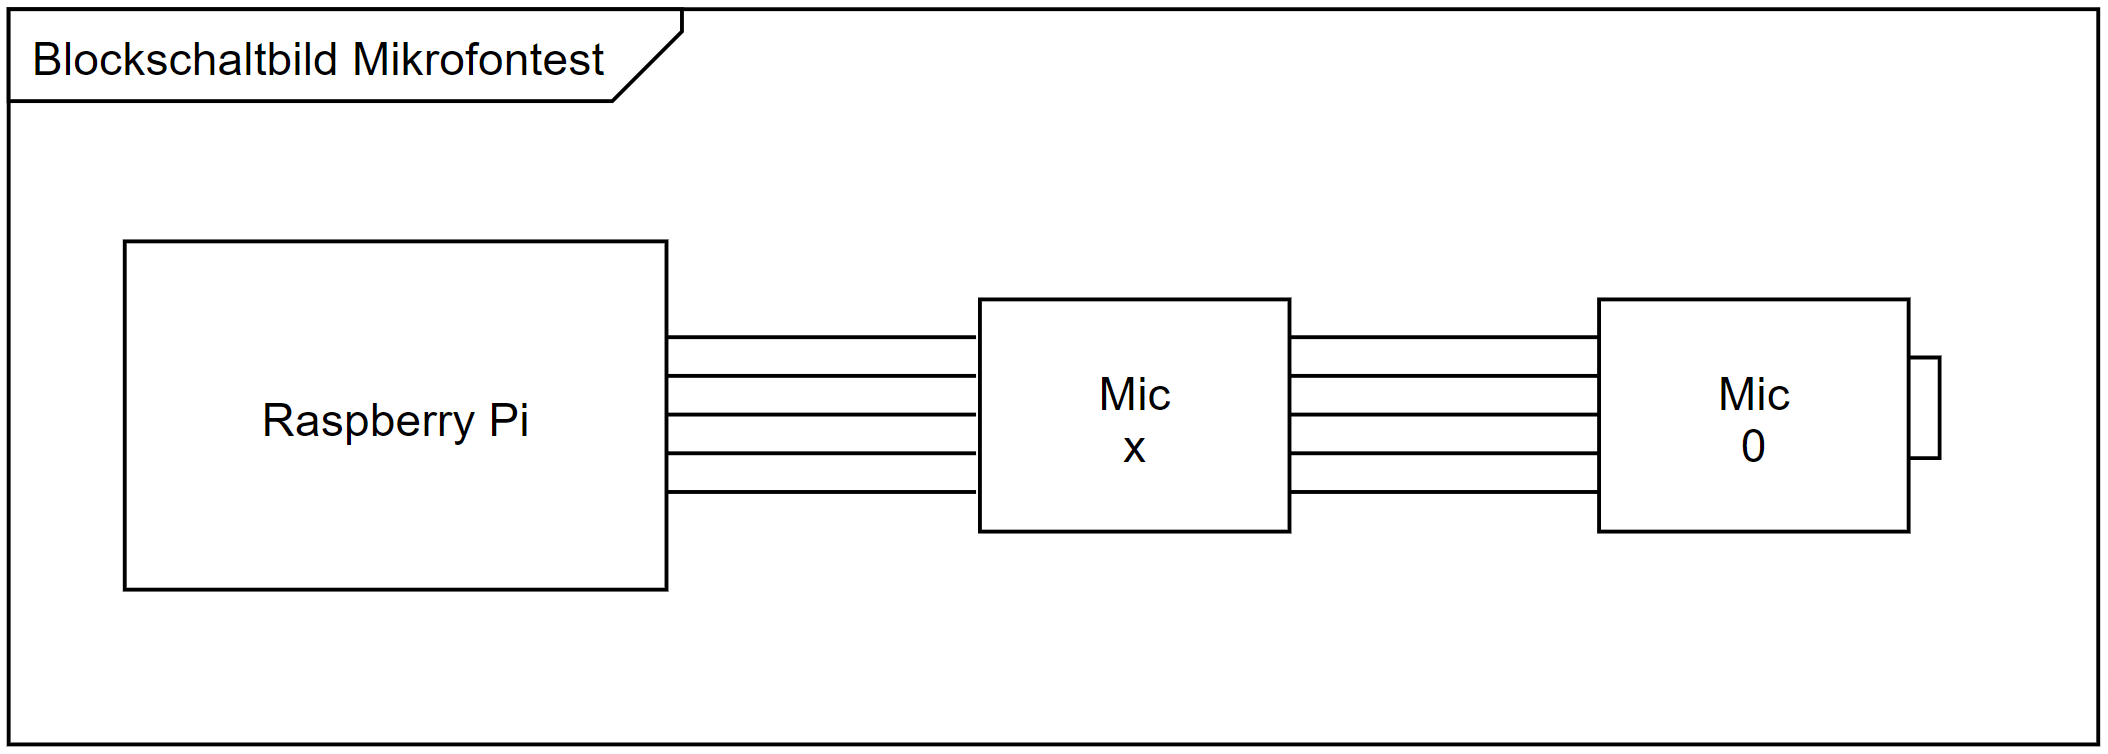
\includegraphics[scale=0.1]{Sections/Tests/BlockbildMikroTest}
	\end{center}
	\caption{Blockbild Mikro Test}
	\label{fig:BlockbildMikroTest}
\end{figure}

Mit dem Skript \glqq RecordMicToRAM\grqq\ wurden die Daten des Mikrofonpaar eingelesen und auf ihre Vollständigkeit überprüft. Es wird eine .txt-Datei erzeugt. In dieser Datei sind 7 Spalten und für das entsprechende Mikrofon tauchen bei erfolgreichem Durchlauf Messwerte auf. So konnte die korrekte Funktion der einzelnen Mikrofone garantiert werden.

\begin{tabularx}{\columnwidth}{|p{4cm}|X|}
	\hline
	\textbf{Abschnitt} & \textbf{Inhalt}\\
	\hline
	\textbf{Name} & Mikrofonfunktionstest\\
	\hline
	\textbf{Autor(en)} & Philipp Otto\\
	\hline
	\textbf{Priorität} & hoch\\	
	\hline	
	\textbf{Kritikalität} & hoch\\
	\hline
	%	\textbf{Quelle} & \\
	%	\hline
	\textbf{Verantwortlicher} & Philipp Otto\\
	\hline
	\textbf{Kurzbeschreibung} & Mit diesem Test soll die fehlerfreie Funktion der Mikrofone getestet werden\\
	\hline
	\textbf{Auslösendes Ereignis} & Eingabe Konsole: \glqq sudo ./RecordMicToRAM\grqq\\
	\hline
	\textbf{Akteure} & Mirkofonpaar, Rasberry Pi, Jumperkabel\\
	\hline
	\textbf{Vorbedingung} & Raspberry eingerichtet, Mikrofone und Raspberry mit Kabel verbunden, Raspberry eingeschaltet\\
	\hline
	\textbf{Nachbedingung} & \glqq RecordMicToRAM\grqq\ beendet,
	Prüfung der .txt-Datei ist erfolgt
	\\
	\hline
	\textbf{Ergebnis} & .txt- Datei erstellt\\
	\hline
	\textbf{Hauptszenario} & \begin{description}[font=\normalfont]
		\item[1.] Über die Konsoleneingabe wird das Programm gestartet
		\item[2.] Das Programm zeichnet ca. 8 Sekunden lang den Aikrofonausgang auf
		\item[3.] Das Programm erstellt eine .txt-Datei mit allen Messwerten
		\item[4.] Die .txt-Datei wird auf Vollständigkeit überprüft
	\end{description}\\
	\hline
	\textbf{Alternativszenario} & \begin{description}[font=\normalfont]
		\item[4.b] Die .txt-Datei enthält keine Messwerte
		\item[4.c] Kabelverbindung wird überprüft
	\end{description}\\
	%	\hline
	%	\textbf{Ausnahmeszenario} & \\
	%	\hline
	%	\textbf{Qualitäten} & \\
	\hline
\end{tabularx}
\captionof{table}{Mikrofonfunktionstest}
\label{tab:Mikrofonfunktionstest}

\subsection{Hardware Test}

\subsection{Kabelfunktionstest 1}

In einem ersten Entwicklungsschritt wurde das gesamte Mikrofonarray mit großzügig dimensionierten Verbindungskabeln (Kabellänge ca. 50 cm) aufgebaut und in Abständen von ungefähr \SI{20}{cm} zueinander platziert. 

\begin{figure}[h]
	\begin{center}
		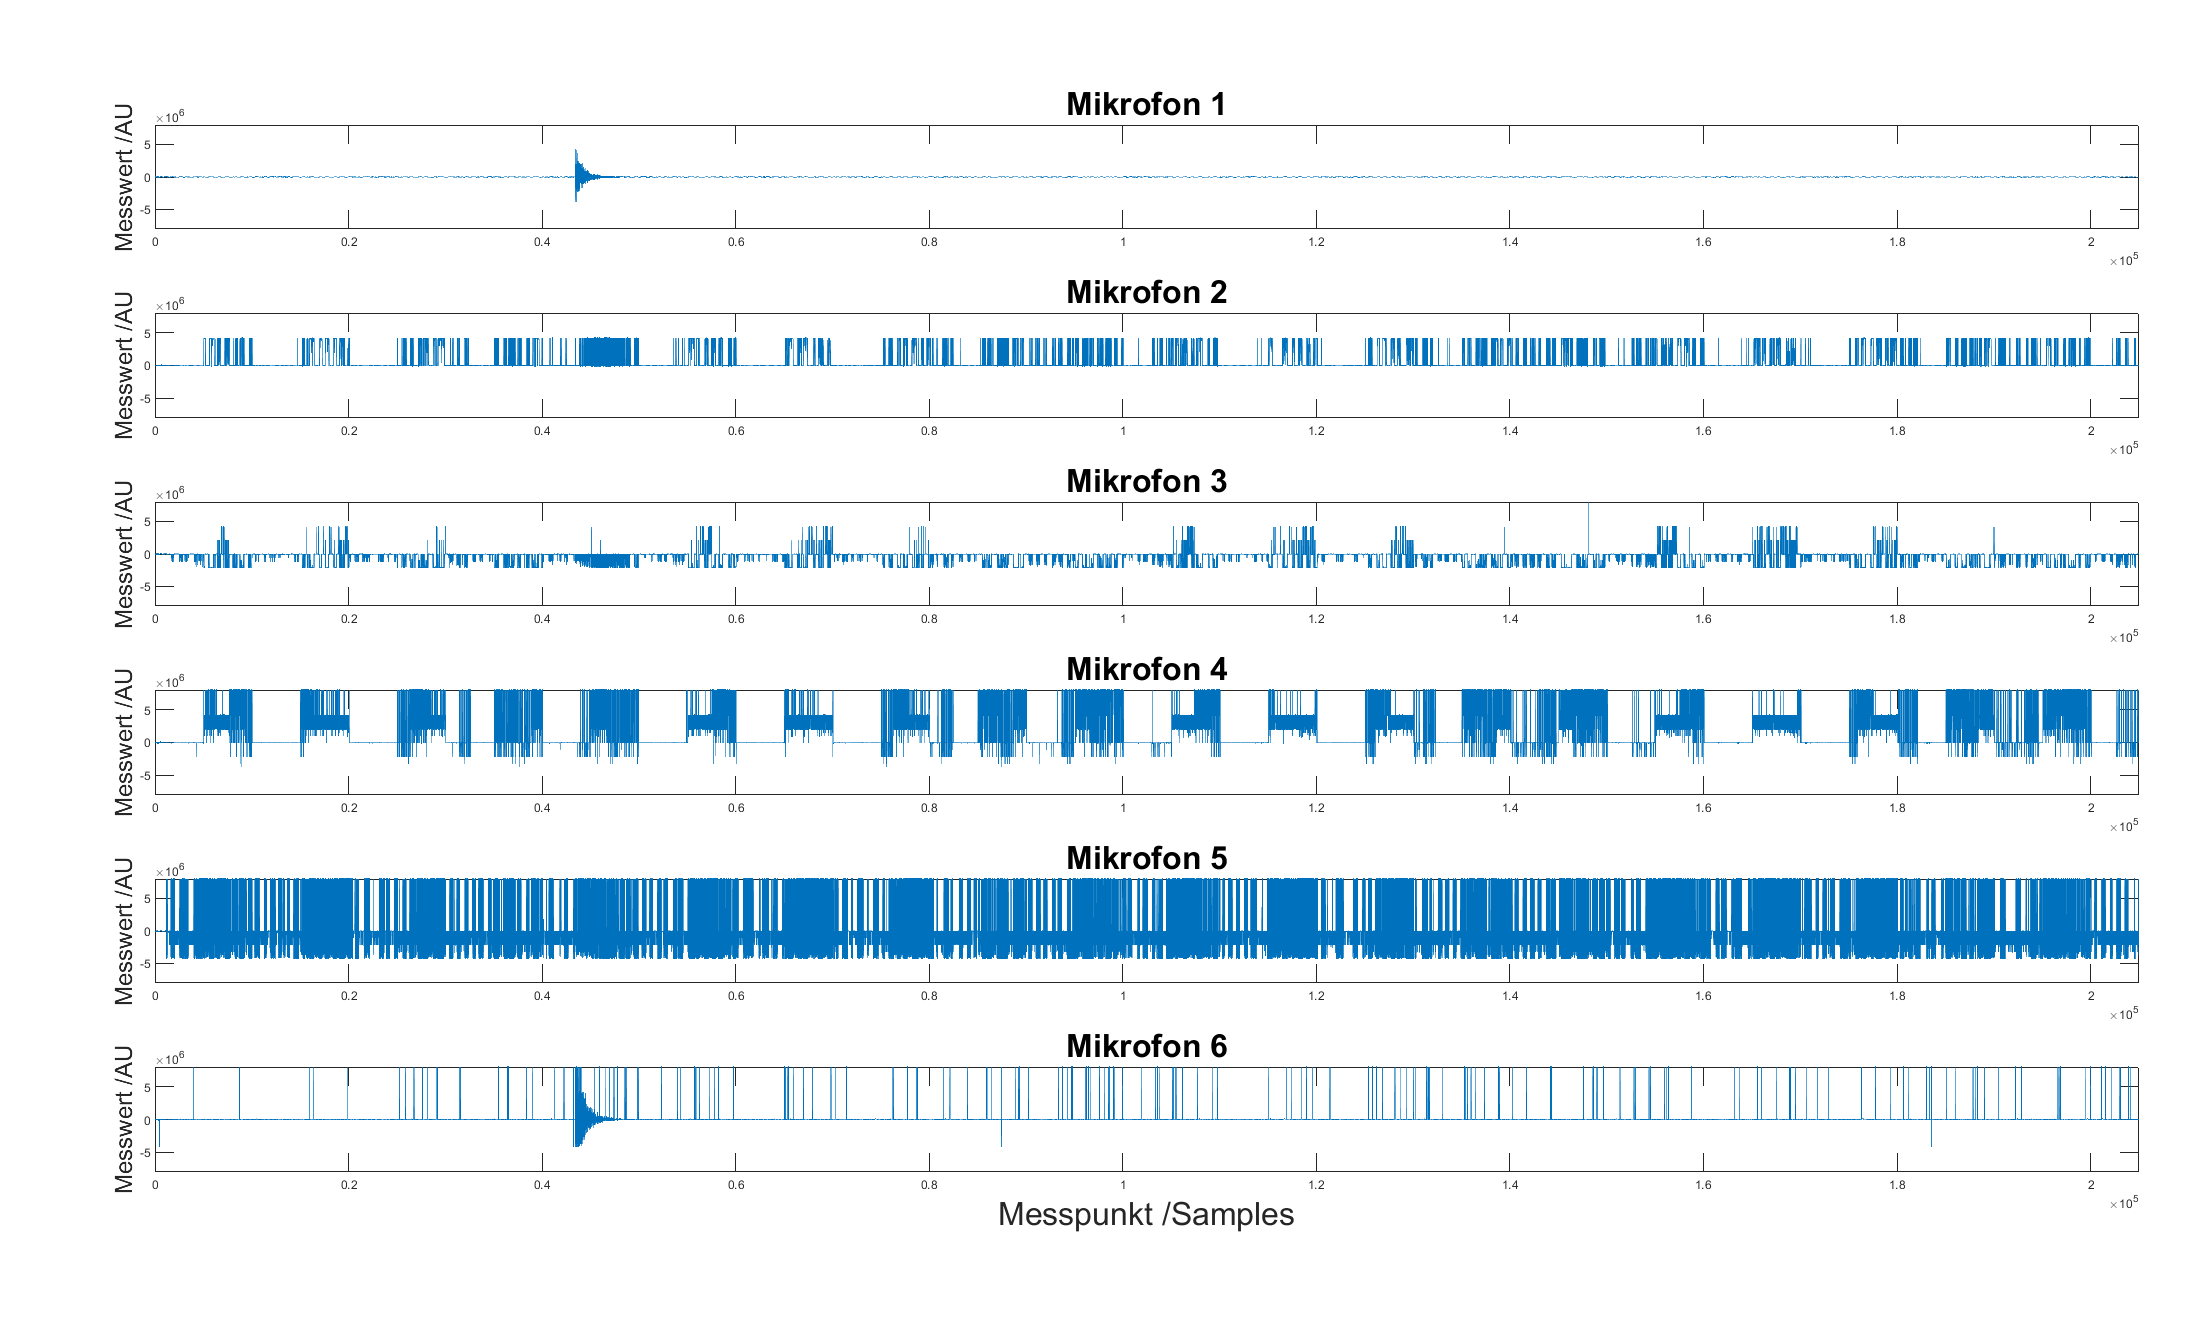
\includegraphics[scale=0.1]{Sections/Tests/Test_1_d}
	\end{center}
	\caption{Kabelfunktionstest 1}
	\label{fig:Test_1_d}
\end{figure}

Die dargestellte Messung wurde über einen Zeitraum von acht Sekunden durchgeführt mit einem Händeklatschen nach ungefähr zwei Sekunden.

Die Erwartungshaltung an die Ergebnisse war ein sauberer Ausschlag der Messwerte bei ungefähr einem Viertel der vergangenen Testzeit mit einem anschließenden Abklingen auf den Umgebungspegel.

Lediglich die Aufzeichnungen aus Mikrofon 1 entsprachen den Erwartungen (Ausschlag bei ca. 40.000 Samples), während die restlichen Mikrofone deutliches Rauschen aufwiesen. In der Aufzeichnung von Mikrofon 3 war selbst das Event (erwartet bei ca. 40.000 Samples) nicht zu erkennen, während auf den anderen Kanälen noch Andeutungen eines stärker verrauschten Bereiches zu erkennen waren. Dieses Verhalten hätte seine Ursache beim Raspberry Pi haben können. Dieser muss für die Taktung der Mikrofone einen SPI-Takt über das gesamte Array treiben können. Mit zunehmender Kabellänge nimmt die Taktsicherheit ab. 

Durch ein Fachgespräch mit Max Weltz schlossen wir auf folgende mögliche Ursachen:

\begin{itemize}
	\item Kabel defekt
	\item SPI-Takt zu hoch
	\item Kabel zu lang
\end{itemize}

Um eine qualitative Ursachensuche vornehmen zu können, beschlossen wir die aufgezählten Ursachen separat zu Untersuchen.

\begin{tabularx}{\columnwidth}{|p{4cm}|X|}
	\hline
	\textbf{Abschnitt} & \textbf{Inhalt}\\
	\hline
	\textbf{Name} & Kabelfunktionstest Nr. 1\\
	\hline
	\textbf{Autor(en)} & Philipp Otto\\
	\hline
	\textbf{Priorität} & hoch\\	
	\hline	
	\textbf{Kritikalität} & hoch\\
	\hline
	%	\textbf{Quelle} & \\
	%	\hline
	\textbf{Verantwortlicher} & Philipp Otto\\
	\hline
	\textbf{Kurzbeschreibung} & Mit diesem Test soll die fehlerfreie Funktion der Kabel getestet werden\\
	\hline
	\textbf{Auslösendes Ereignis} & Eingabe Konsole: \glqq sudo ./RecordMicToRAM\grqq\\
	\hline
	\textbf{Akteure} & gesamtes Mikrofonarray, Raspberry Pi, Kabel (lang)\\
	\hline
	\textbf{Vorbedingung} & Das Array ist vollständig mit Kabeln und Raspberry verbunden, Raspberry eingeschaltet\\
	\hline
	\textbf{Nachbedingung} & Messwerte grafisch auf Plausibilität überprüft
	\\
	\hline
	\textbf{Ergebnis} & Plot der Messwerte\\
	\hline
	\textbf{Hauptszenario} & \begin{description}[font=\normalfont]
		\item[1.] Über die Konsoleneingabe wird das Programm gestartet
		\item[2.] Das Programm zeichnet ca. 8 Sekunden lang den Mikrofonausgang auf
		\item[3.] Das Programm erstellt eine .txt-Datei mit allen Messwerten
		\item[4.] Die .txt-Datei wird mit python-script in korrektes Datenformat gebracht und in .csv konvertiert
		\item[5.] .csv wird mit Matlab eingelesen und geplottet
		\item[6.] Plot wird auf Plausibilität überprüft
	\end{description}\\
	\hline
	\textbf{Alternativszenario} & \begin{description}[font=\normalfont]
		\item[4.b] Die .txt-Datei enthält keine Messwerte
		\item[4.c] Kabelverbindung wird überprüft
		\item[6.b] Plot weist fehlerhafte Messwerte auf
	\end{description}\\
	%\hline
	%	\textbf{Ausnahmeszenario} & \\
	%	\hline
	%	\textbf{Qualitäten} & \\
	\hline
\end{tabularx}
\captionof{table}{ Kabelfunktionstest Nr. 1}
\label{tab: Kabelfunktionstest Nr. 1}

\subsection{Kabelfunktionstest 2}

In einer zweiten Iteration wurde das System umkonfiguriert, sodass jetzt mit einem SPI-Takt von \SI{3,9}{MHz} und nicht wie ursprünglich mit \SI{7,8}{MHz} gearbeitet wird. 

\begin{figure}[h]
	\begin{center}
		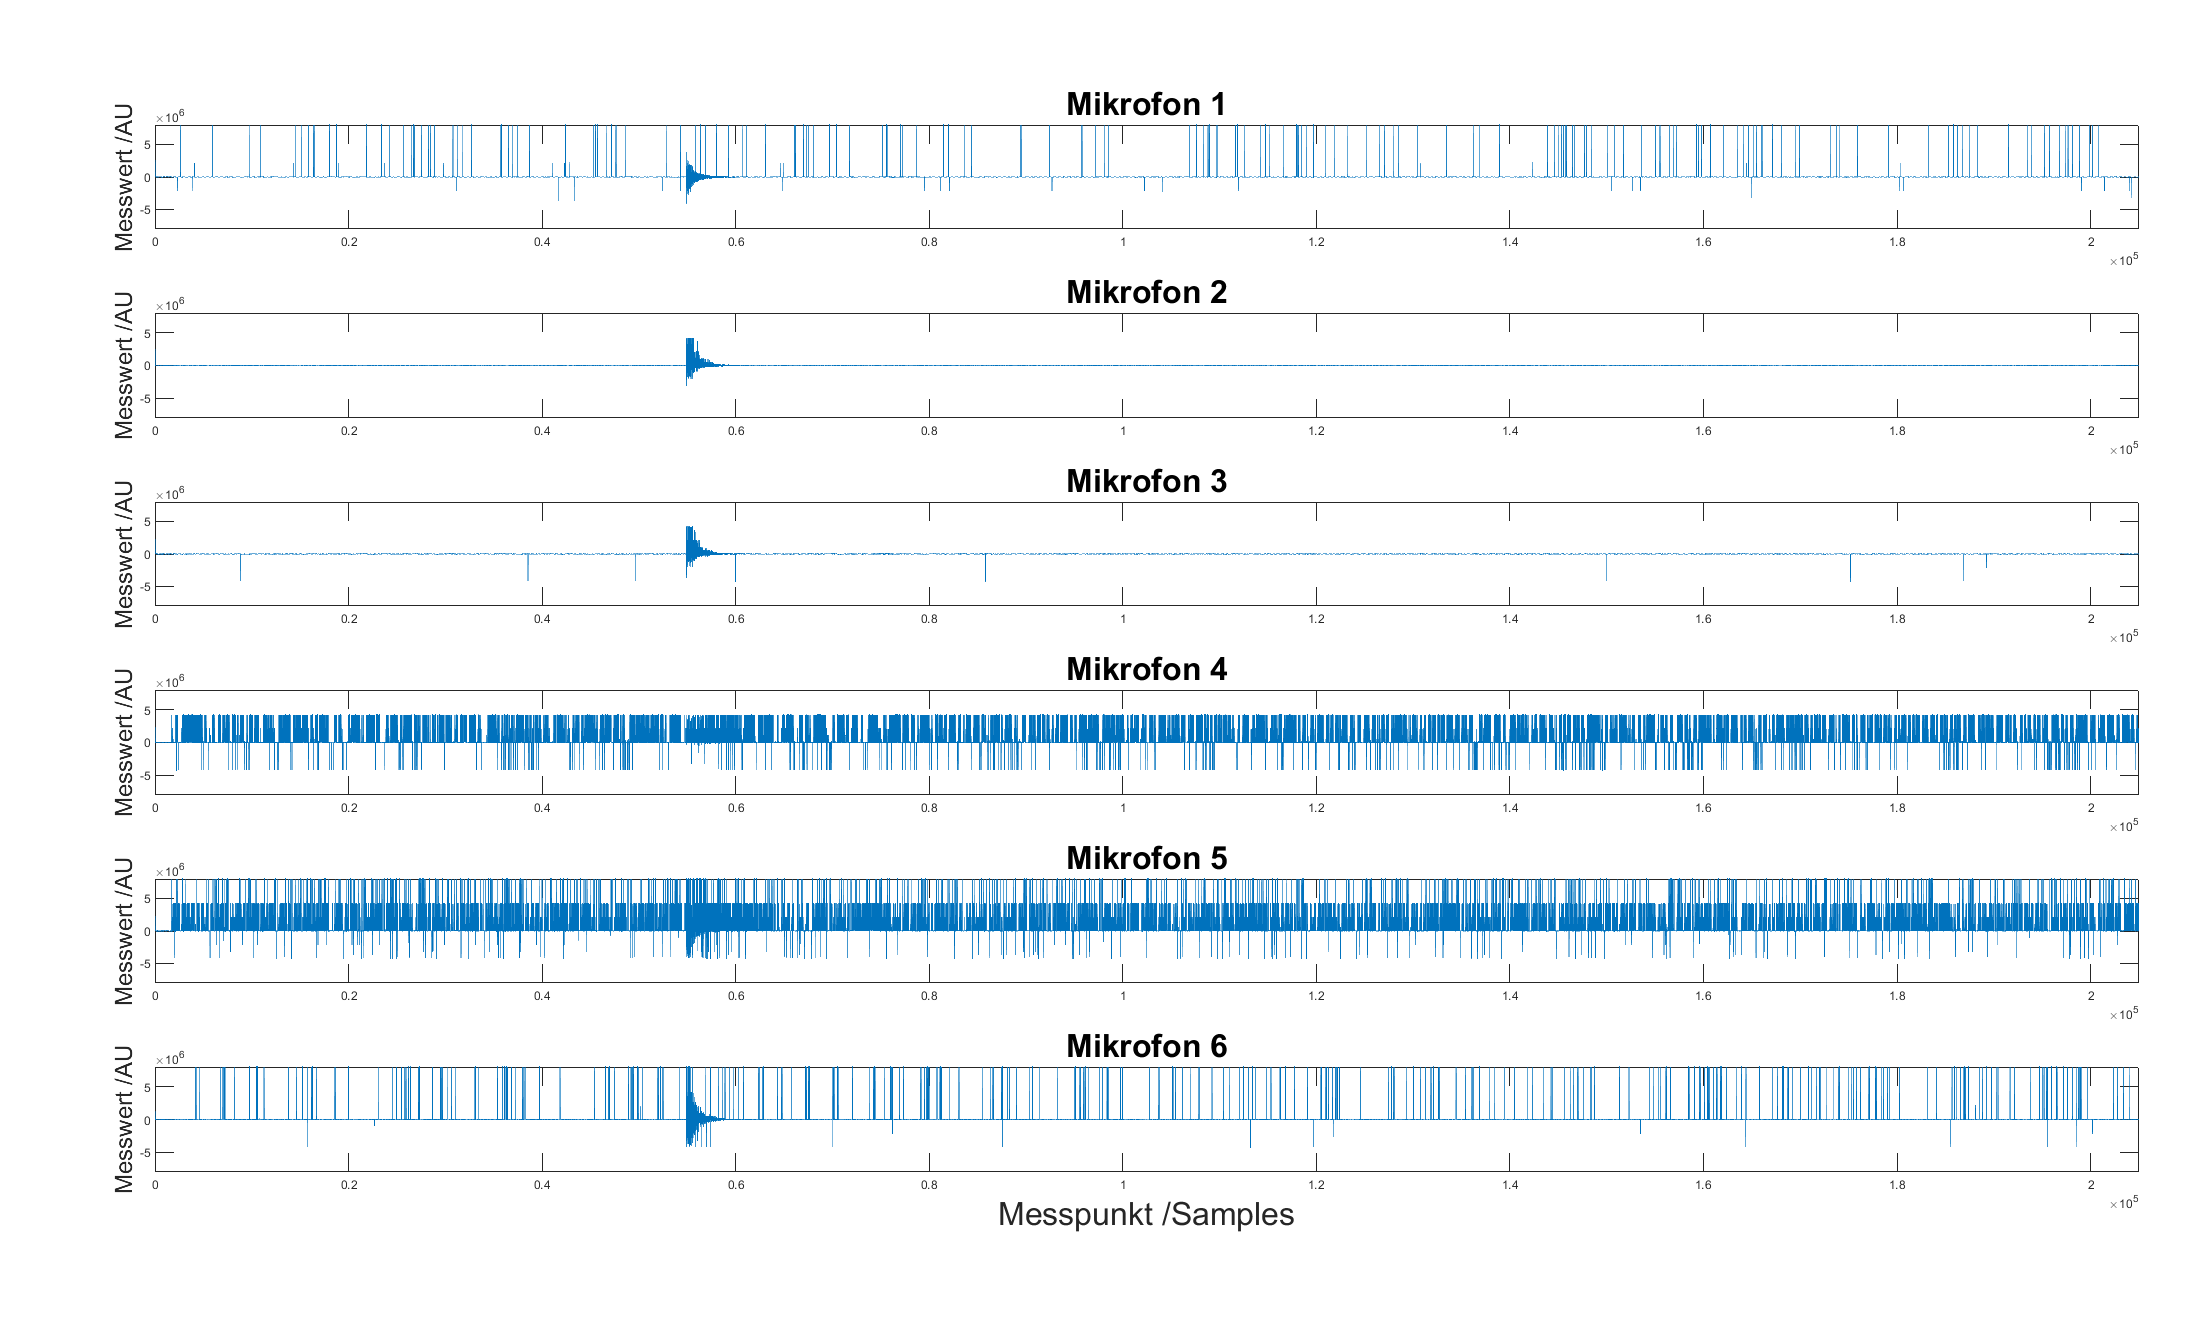
\includegraphics[scale=0.1]{Sections/Tests/Test_2_d}
	\end{center}
	\caption{Kabelfunktionstest 2}
	\label{fig:Test_2_d}
\end{figure}

Für diese Konfiguration wurde die gleiche Testmethode verwendet und es ist zu erkennen, dass die Messungen nun deutlich weniger verrauscht waren. Dennoch sind immer wieder bit-shift Fehler zu erkennen, die das Messergebnis zu bestimmten Schwellenwerten springen lässt. Die Messungen waren somit immer noch zu stark verrauscht und für eine Verwendung unbrauchbar. 

Eine reine Reduzierung des verwendeten SPI-Takts hat das Problem also noch nicht vollständig gelöst.

\begin{tabularx}{\columnwidth}{|p{4cm}|X|}
	\hline
	\textbf{Abschnitt} & \textbf{Inhalt}\\
	\hline
	\textbf{Name} & Kabelfunktionstest Nr. 2\\
	\hline
	\textbf{Autor(en)} & Philipp Otto\\
	\hline
	\textbf{Priorität} & hoch\\	
	\hline	
	\textbf{Kritikalität} & hoch\\
	\hline
	%	\textbf{Quelle} & \\
	%	\hline
	\textbf{Verantwortlicher} & Philipp Otto\\
	\hline
	\textbf{Kurzbeschreibung} &Mit diesem Test soll die fehlerfreie Funktion der Kabel bei halbiertem SPI-Takt getestet werden\\
	\hline
	\textbf{Auslösendes Ereignis} & Eingabe Konsole: \glqq sudo ./RecordMicToRAM64\grqq\\
	\hline
	\textbf{Akteure} & gesamtes Mikrofonarray, Raspberry Pi, Kabel (lang)\\
	\hline
	\textbf{Vorbedingung} & Das Array ist vollständig mit Kabeln und Raspberry verbunden, Raspberry eingeschaltet\\
	\hline
	\textbf{Nachbedingung} & Messwerte grafisch auf Plausibilität überprüft
	\\
	\hline
	\textbf{Ergebnis} & Plot der Messwerte\\
	\hline
	\textbf{Hauptszenario} & \begin{description}[font=\normalfont]
		\item[1.] Über die Konsoleneingabe wird das Programm gestartet
		\item[2.] Das Programm zeichnet ca. 8 Sekunden lang den Mikrofonausgang auf
		\item[3.] Das Programm erstellt eine .txt-Datei mit allen Messwerten
		\item[4.] Die .txt-Datei wird mit python-script in korrektes Datenformat gebracht und in .csv konvertiert
		\item[5.] .csv wird mit Matlab eingelesen und geplottet
		\item[6.] Plot wird auf Plausibilität überprüft
	\end{description}\\
	\hline
	\textbf{Alternativszenario} & \begin{description}[font=\normalfont]
		\item[4.b] Die .txt-Datei enthält keine Messwerte
		\item[4.c] Kabelverbindung wird überprüft
		\item[6.b] Plot weist fehlerhafte Messwerte auf
	\end{description}\\
	%\hline
	%	\textbf{Ausnahmeszenario} & \\
	%	\hline
	%	\textbf{Qualitäten} & \\
	\hline
\end{tabularx}
\captionof{table}{ Kabelfunktionstest Nr. 2}
\label{tab: Kabelfunktionstest Nr. 2}

\subsection{Kabelfunktionstest 3}

In der nächsten Anpassung wurde die Kabellänge der Mikrofonkabel auf nun ca. \SI{25}{cm} reduziert mit der Erwartung, dass die Taktsicherheit über die gesamte Kabellänge steigen sollte.

\begin{figure}[h]
	\begin{center}
		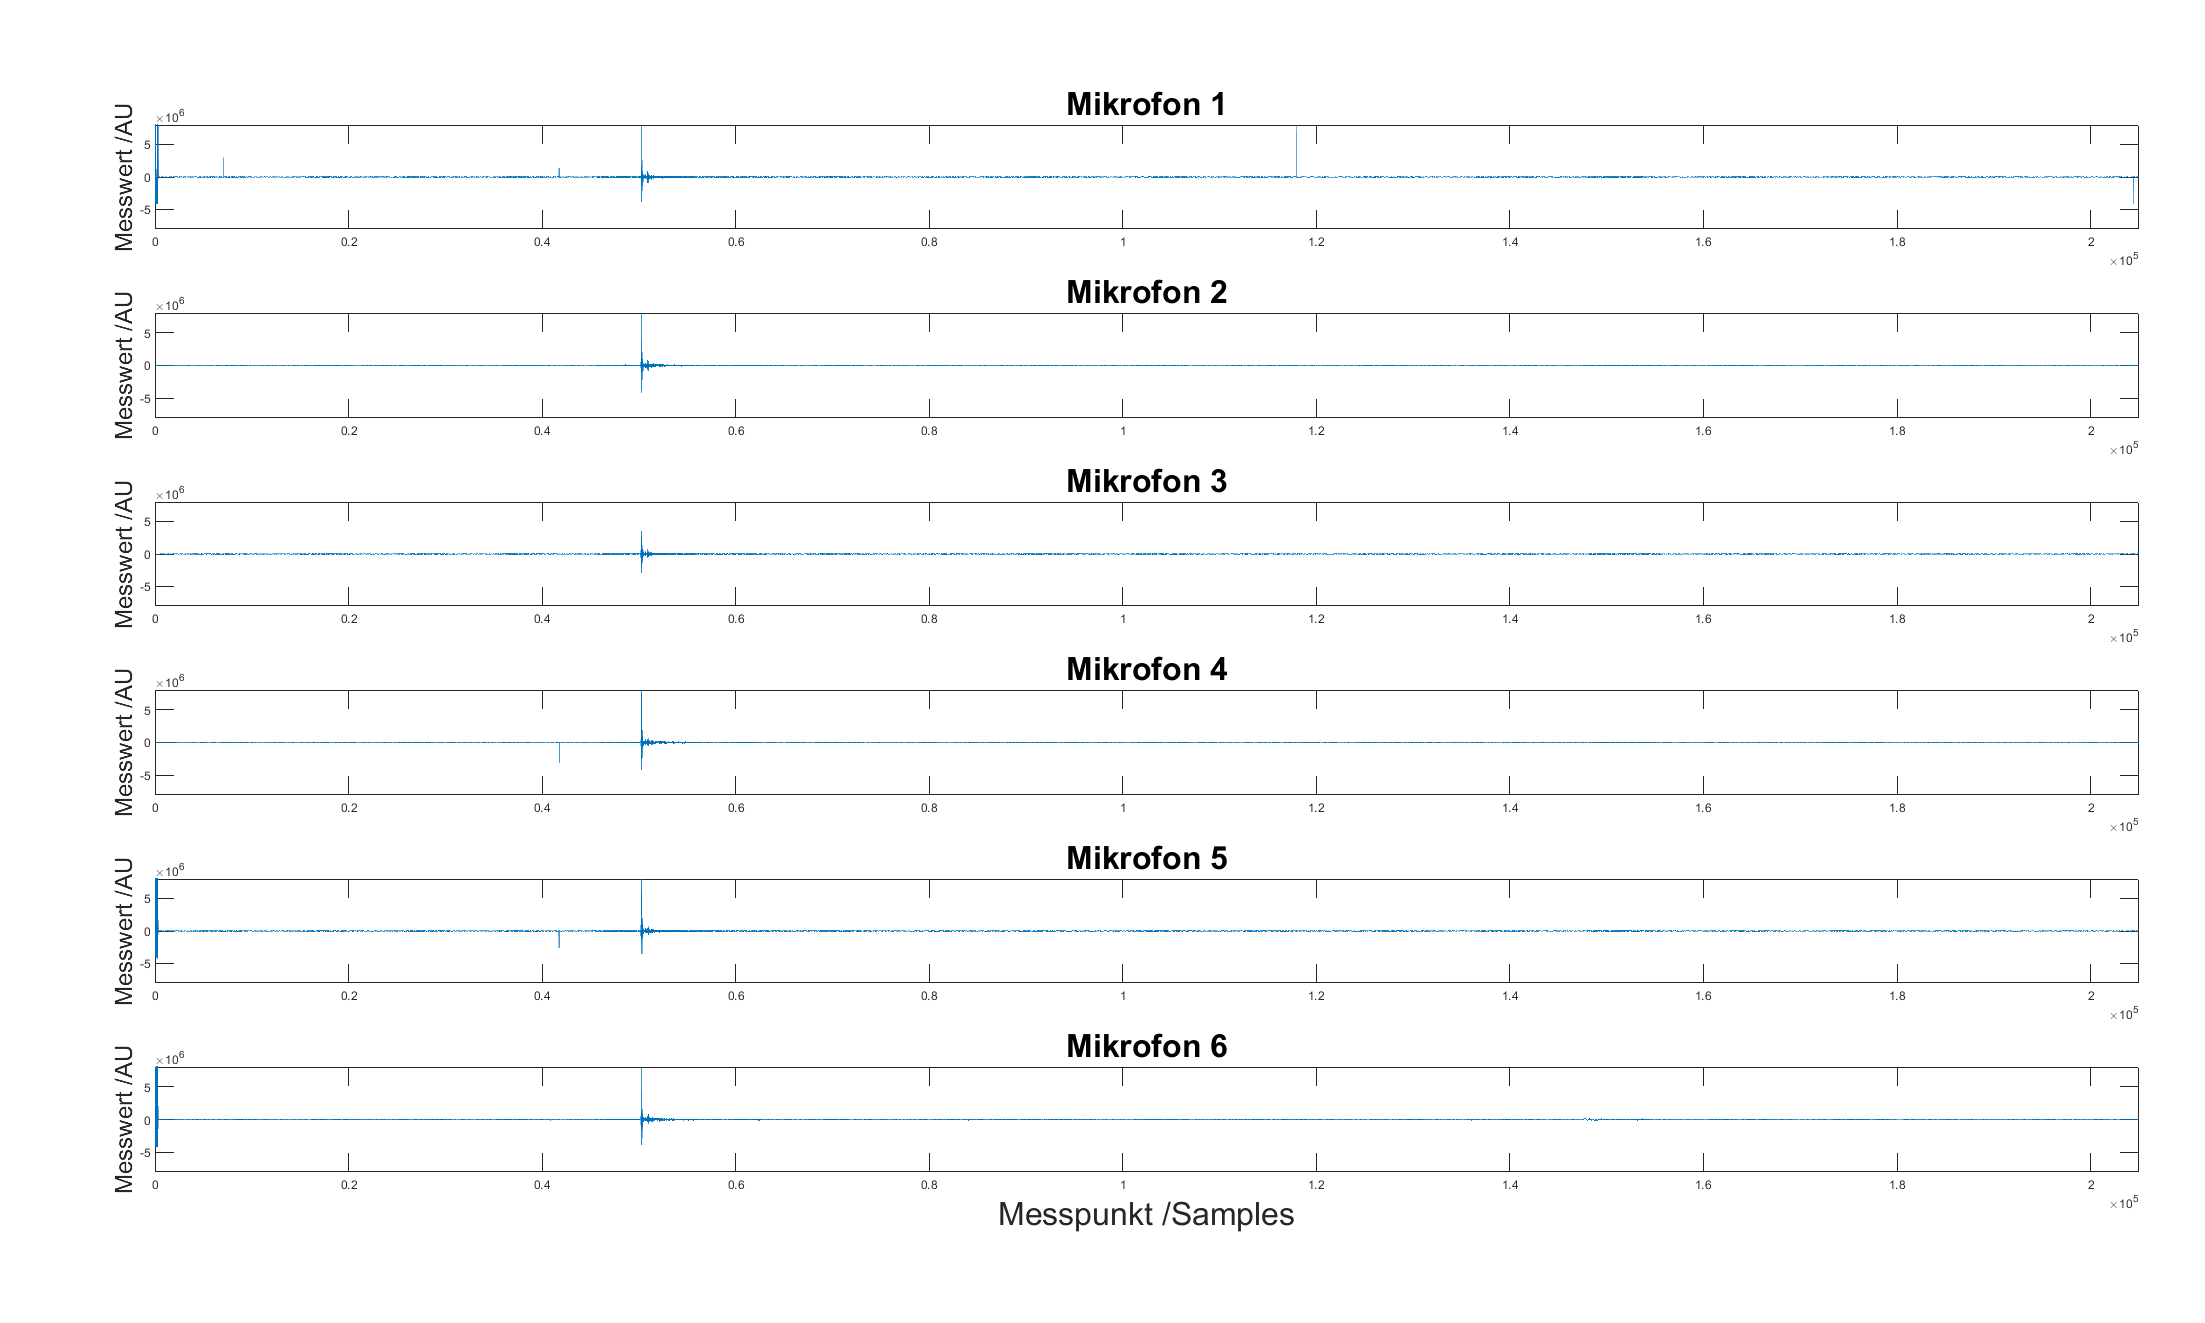
\includegraphics[scale=0.1]{Sections/Tests/Test_3_d}
	\end{center}
	\caption{Kabelfunktionstest 3}
	\label{fig:Test_3_d}
\end{figure}

Die nun durchgeführte Messung wies das gewünschte, rauschfreie Verhalten der Messwerte auf allen Kanälen auf. Die Kabel wurden somit in Bezug auf die Datenübertragung hinreichend auf die Funktion überprüft. 

\begin{tabularx}{\columnwidth}{|p{4cm}|X|}
	\hline
	\textbf{Abschnitt} & \textbf{Inhalt}\\
	\hline
	\textbf{Name} & Kabelfunktionstest Nr. 2\\
	\hline
	\textbf{Autor(en)} & Philipp Otto\\
	\hline
	\textbf{Priorität} & hoch\\	
	\hline	
	\textbf{Kritikalität} & hoch\\
	\hline
	%	\textbf{Quelle} & \\
	%	\hline
	\textbf{Verantwortlicher} & Philipp Otto\\
	\hline
	\textbf{Kurzbeschreibung} & Mit diesem Test soll die fehlerfreie Funktion der Kabel bei halbiertem SPI-Takt und kürzeren Kabeln getestet werden\\
	\hline
	\textbf{Auslösendes Ereignis} & Eingabe Konsole: \glqq sudo ./RecordMicToRAM64\grqq\\
	\hline
	\textbf{Akteure} & gesamtes Mikrofonarray, Raspberry Pi, Kabel (kurz)\\
	\hline
	\textbf{Vorbedingung} & Das Array ist vollständig mit Kabeln und Raspberry verbunden, Raspberry eingeschaltet\\
	\hline
	\textbf{Nachbedingung} & Messwerte grafisch auf Plausibilität überprüft
	\\
	\hline
	\textbf{Ergebnis} & Plot der Messwerte\\
	\hline
	\textbf{Hauptszenario} & \begin{description}[font=\normalfont]
		\item[1.] Über die Konsoleneingabe wird das Programm gestartet
		\item[2.] Das Programm zeichnet ca. 8 Sekunden lang den Mikrofonausgang auf
		\item[3.] Das Programm erstellt eine .txt-Datei mit allen Messwerten
		\item[4.] Die .txt-Datei wird mit python-script in korrektes Datenformat gebracht und in .csv konvertiert
		\item[5.] .csv wird mit Matlab eingelesen und geplottet
		\item[6.] Plot wird auf Plausibilität überprüft
	\end{description}\\
	\hline
	\textbf{Alternativszenario} & \begin{description}[font=\normalfont]
		\item[4.b] Die .txt-Datei enthält keine Messwerte
		\item[4.c] Kabelverbindung wird überprüft
		\item[6.b] Plot weist fehlerhafte Messwerte auf
	\end{description}\\
	%\hline
	%	\textbf{Ausnahmeszenario} & \\
	%	\hline
	%	\textbf{Qualitäten} & \\
	\hline
\end{tabularx}
\captionof{table}{ Kabelfunktionstest Nr. 3}
\label{tab: Kabelfunktionstest Nr. 3}

\subsection{Algorithmustest}

Im nächsten Testschritt wurde das Gesamtsystem in einer den Anforderungen entsprechenden Umgebungssituation Situation getestet. Das bedeutet das System wurde auf einem Stativ in fast vollständig aufgebautem Zustand im freien, in einer echoreduzierten Umgebung betrieben.

\begin{figure}[h]
	\begin{center}
		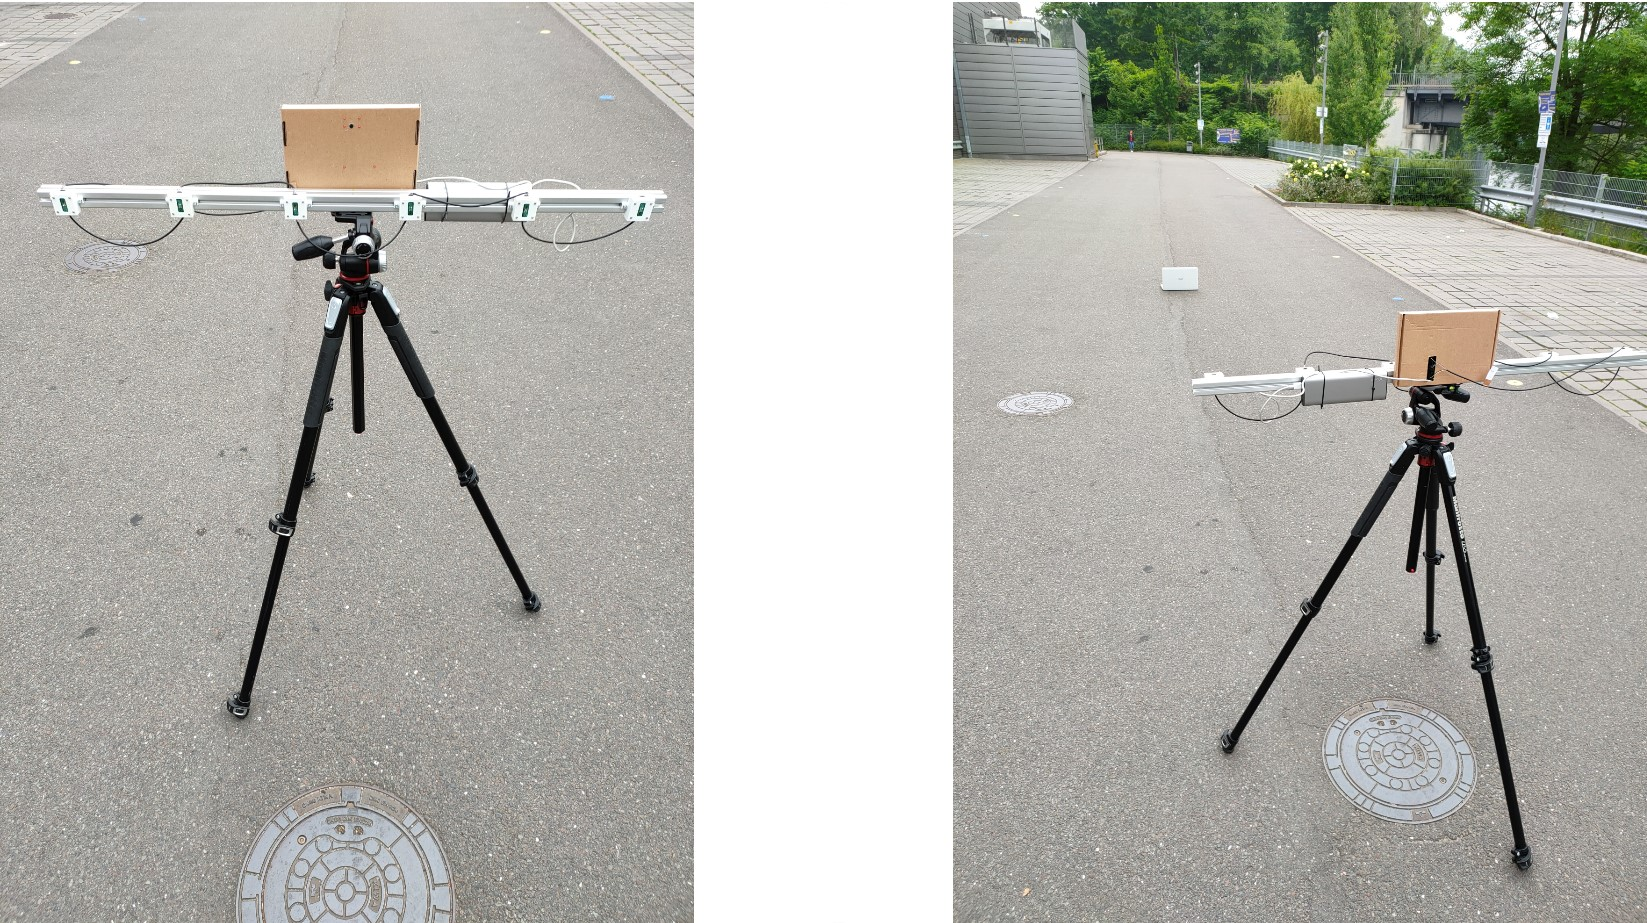
\includegraphics[scale=0.1]{Sections/Tests/Gesamtaufbau}
	\end{center}
	\caption{provisorischer Gesamtaufbau}
	\label{fig:Test_4}
\end{figure}

Zunächst wurde erneut eine Messung über eine Dauer von acht Sekunden durchgeführt und wieder nach ungefähr zwei Sekunden ein Händeklatschen in einer Distanz von ca. \SI{15}{m} aufgezeichnet.

Die Aufgezeichneten Werte  der Messungen, also 205000 Messwerte pro Mikrofon wurden im Anschluss in Matlab mit dem gleichen Algorithmus ausgewertet, der auch Systemintern verwendet wird. Die Lokalisierung ergab folgendes Bild:

\begin{figure}[h]
	\begin{center}
		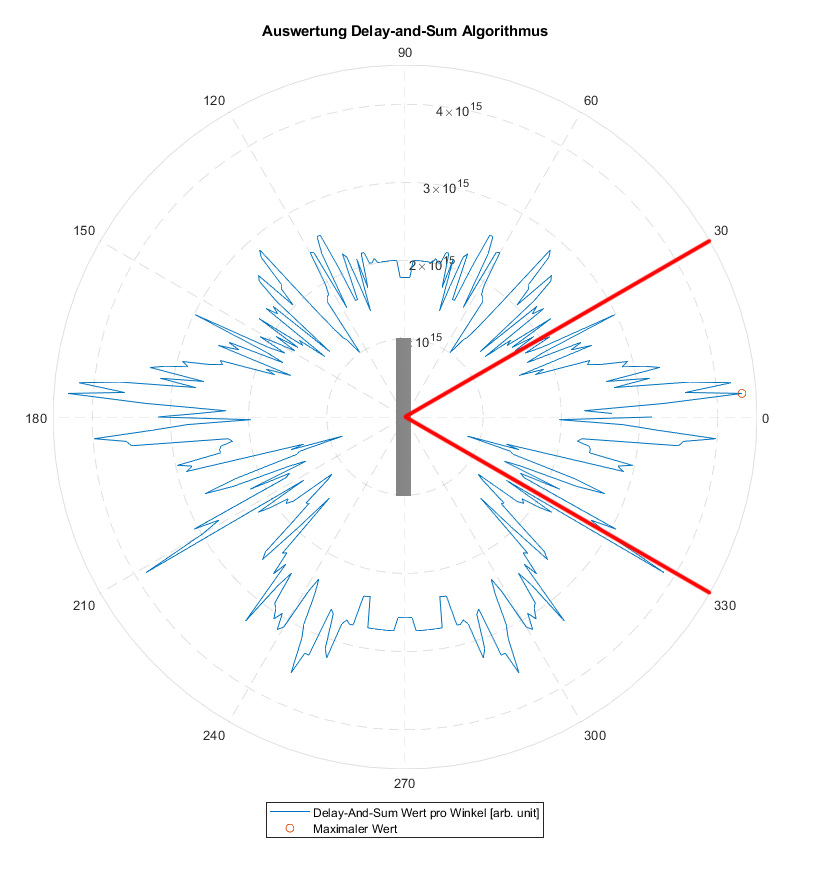
\includegraphics[scale=0.1]{Sections/Tests/Test_6_b}
	\end{center}
	\caption{Auswertung Delay-and-Sum Algorithmus}
	\label{fig:Test_6_b}
\end{figure}

Wie zu erwarten ist das Bild der Lokalisierung Achsensymmetrisch entlang der vertikalen, da unser definiertes Koordinatensystem entsprechend rotiert ist. Betrachtet wird in der Auswertung nur der Bereich von \ang{0} - \ang{30} und \ang{330} - \ang{360}, da dieser Winkelbereich ebenfalls von der Systemkamera abgedeckt wird. Ein Ergebnis der Lokalisierung nahe \ang{0} legt also ein Eventursprung frontal des Systems und somit mittig im Bild nahe. Das Ergebnis der Berechnung stimmte ebenfalls mit den Erwartungen überein, da das Geräusch ebenfalls ungefähr frontal vor dem System erzeugt wurde.

\begin{tabularx}{\columnwidth}{|p{4cm}|X|}
	\hline
	\textbf{Abschnitt} & \textbf{Inhalt}\\
	\hline
	\textbf{Name} & Algorithmus-Test (Matlab)\\
	\hline
	\textbf{Autor(en)} & Philipp Otto\\
	\hline
	\textbf{Priorität} & hoch\\	
	\hline	
	\textbf{Kritikalität} & hoch\\
	\hline
	%	\textbf{Quelle} & \\
	%	\hline
	\textbf{Verantwortlicher} & Philipp Otto\\
	\hline
	\textbf{Kurzbeschreibung} & Mit diesem Test soll die fehlerfreie Funktion des Lokalisierungs-algorithmus getestet werden\\
	\hline
	\textbf{Auslösendes Ereignis} & \glqq sudo ./RecordMicToRAM64\grqq\\
	\hline
	\textbf{Akteure} & gesamtes Mirkofonarray, Rasberry Pi, Kabel(kurz)\\
	\hline
	\textbf{Vorbedingung} & Das System ist vollständig montiert, 
	Raspberry eingeschaltet\\
	\hline
	\textbf{Nachbedingung} & Lokalisierungsergebnisse grafisch auf Plausibilität überprüft.\\
	\hline
	\textbf{Ergebnis} & Plot der Lokalisierungsergebnisse\\
	\hline
	\textbf{Hauptszenario} & \begin{description}[font=\normalfont]
		\item[1.] Über die Konsoleneingabe wird das Programm gestartet
		\item[2.] Das Programm zeichnet ca. 8 Sekunden lang den Mikrofonausgang auf
		\item[3.] Das Programm erstellt eine .txt-Datei mit allen Messwerten
		\item[4.] Die .txt-Datei wird mit python Skript in korrektes Datenformat gebracht und in .csv konvertiert
		\item[5.] .csv wird in Matlab eingelesen
		\item[6.] Lokalisierung wird mithilfe des Skripts \glqq testDelayAndSum.m\grqq\ berechnet und geplottet
		\item[7.] Plot wird auf Plausibilität überprüft
	\end{description}\\
	\hline
	\textbf{Alternativszenario} & \begin{description}[font=\normalfont]
		\item[7.b] Lokalisierung entspricht nicht dem erwarteten Winkelbereich
		\item[6.c] Lokalisierung ist uneindeutig
		\item[8.] Messung wird in anderem Umfeld wiederholt
	\end{description}\\
	\hline
	%	\textbf{Ausnahmeszenario} & \\
	%	\hline
	%	\textbf{Qualitäten} & \\
	%	\hline
\end{tabularx}
\captionof{table}{Algorithmus-Test (Matlab)}
\label{tab:Algorithmus_Test_Matlab}


\subsection{Gesamt-Funktionstest}

Im nächsten Test wurde das System wie bereits im Kapitel \glqq Bedienung\grqq\ beschrieben betrieben. 

Auch hier wurde das System wieder in einer anforderungsähnlichen Umgebungssituation aufgebaut.

\begin{figure}[h]
	\begin{center}
		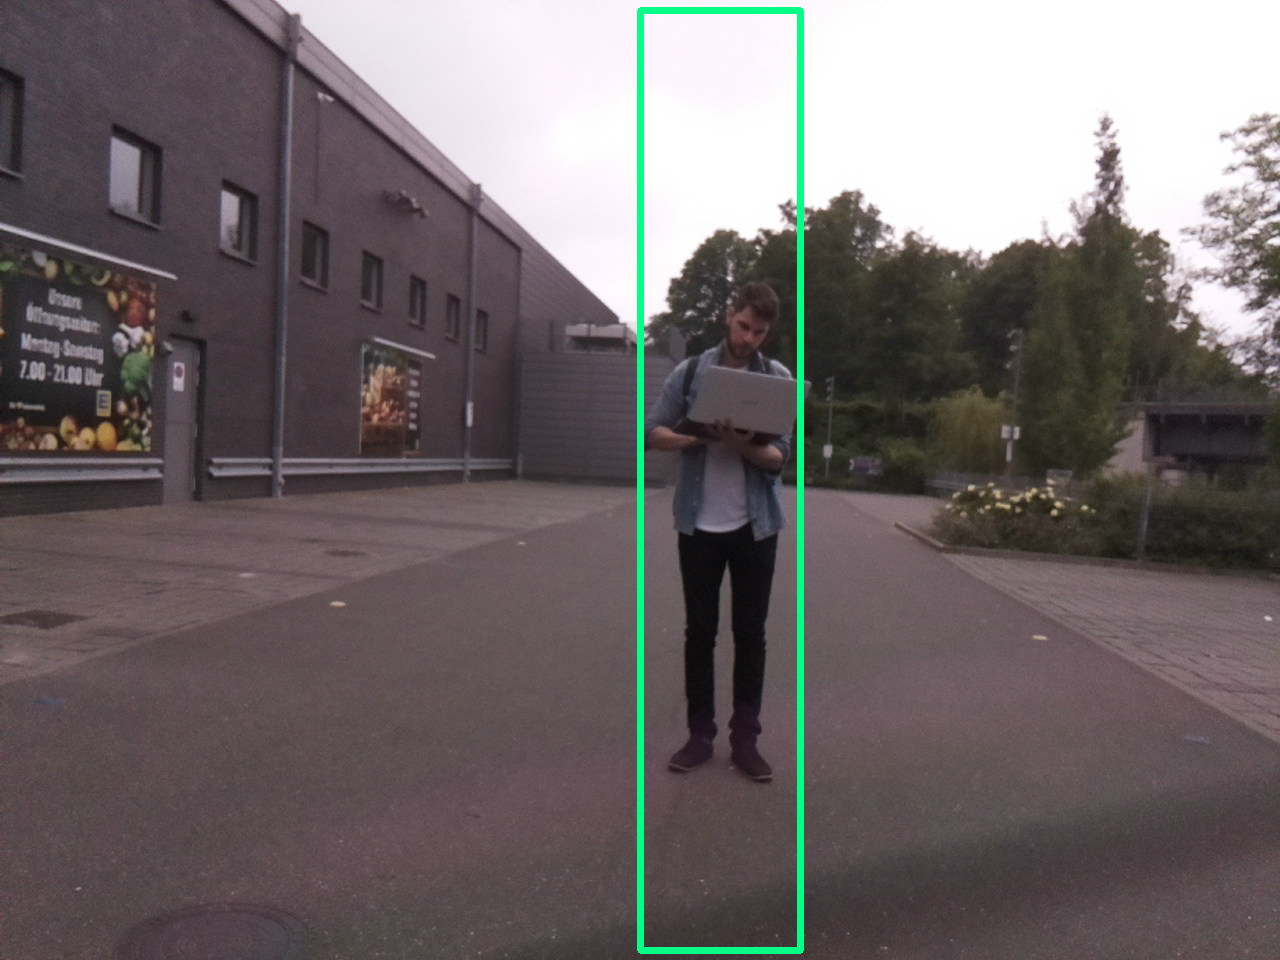
\includegraphics[scale=0.1]{Sections/Tests/Test_7}
	\end{center}
	\caption{erfolgreicher Gesamt-Funktionstest}
	\label{fig:Test_7}
\end{figure}

In diesem Test wurde der eigentliche Dauerbetrieb des Systems getestet. Das bedeutet, das System lief endlos, bis es durch den Nutzer abgebrochen wurde und durch das Programm wurden fortlaufende Messdaten ausgewertet. 

Erwartet wurde eine Benachrichtigung des Nutzers über ein erkanntes Event mit des zugehörigen Lokalisierungsergebnis über die Systemkonsole mit einer zugehörigen .png-Datei, auf der das erkannte Segment farblich markiert wurde.

Der Versuch hat gezeigt, dass das System den erhöhten Pegel eines auftretenden Events sehr gut erkennen kann. Zwar kam es immer wieder zu variierenden Verzögerungen in der Anzeige auf der Konsole, aber es wurden dennoch aufeinanderfolgende Events korrekt hintereinander aufgelistet. Der hierzu verwendete Schwellenwert, ab dem das System auslösen soll, musste zunächst auf die neue Umgebungssituation und auf die Lautstärke des Events angepasst werden. 

Wie im obigen Bild aufgezeigt, konnte der Ursprungsort des Events korrekt lokalisiert werden. 

Bei wiederholter Testdurchführung kam es allerdings auch immer wieder zu Messungen, die nicht den Erwartungen entsprochen haben.

\begin{figure}[h]
	\begin{center}
		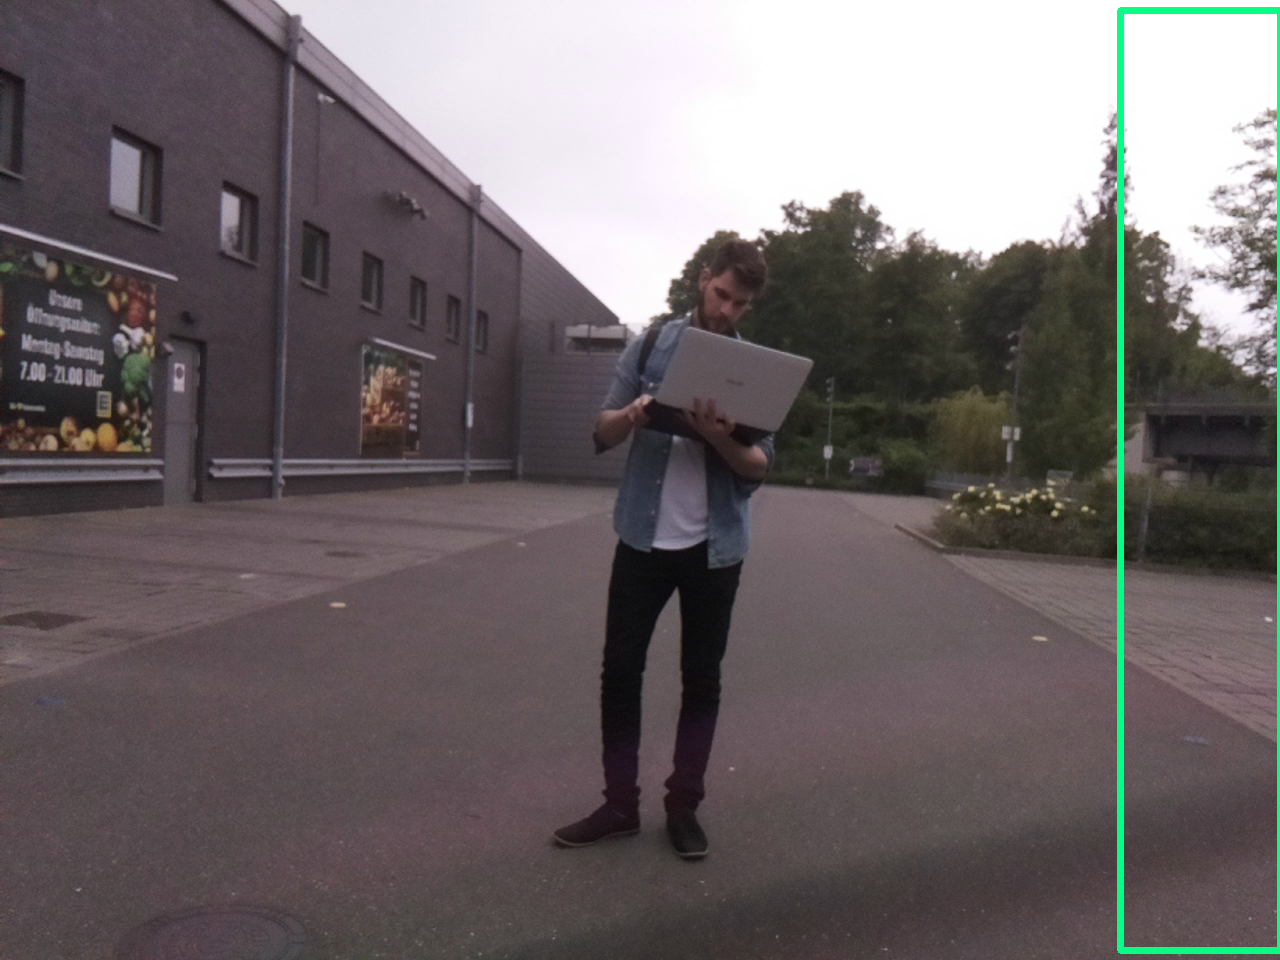
\includegraphics[scale=0.1]{Sections/Tests/Test_8}
	\end{center}
	\caption{unerfolgreicher Gesamt-Funktionstest}
	\label{fig:Test_8}
\end{figure}

Obwohl sich der Ursprungsort des Events ungefähr in der Bildmitte befand, wurde der rechte Bildrand als Ursprung lokalisiert. 

Durch die Fehllokalisierung trat darüber hinaus auch der Fall auf, dass das Event zwar korrekt erkannt wurde, aber aufgrund des fehlerhaft berechneten Ursprungswinkel wurde das Event als außerhalb des Bildbereiches bewertet und keine Beweisführung durchgeführt. 

Diese Fehlmessung ist wahrscheinlich auf die Tatsache rückzuführen, dass der \glqq Raspberry Pi\grqq\ im laufenden Betrieb des Systems nur eine sehr begrenze Menge an Daten in seinem RAM abspeichern kann. Dadurch waren wir gezwungen die Lokalisierung mit einer deutlich reduzierten Menge an Messwerten durchzuführen. 

Leider war es uns nicht möglich ein Testverfahren zu entwickeln, mit dem sich die Genauigkeit der Lokalisierung qualitativ bewerten lässt, um so ein Minimum an benötigten Messdaten ermitteln zu können. Die verwendete Buffergröße wurde lediglich durch Tests ermittelt.

\begin{tabularx}{\columnwidth}{|p{4cm}|X|}
	\hline
	\textbf{Abschnitt} & \textbf{Inhalt}\\
	\hline
	\textbf{Name} & Gesamt-Funktionstest\\
	\hline
	\textbf{Autor(en)} & Philipp Otto\\
	\hline
	\textbf{Priorität} & hoch\\	
	\hline	
	\textbf{Kritikalität} & hoch\\
	\hline
	%	\textbf{Quelle} & \\
	%	\hline
	\textbf{Verantwortlicher} & Philipp Otto\\
	\hline
	\textbf{Kurzbeschreibung} & Mit diesem Test soll die fehlerfreie Funktion des gesamten Programms getestet werden\\
	\hline
	\textbf{Auslösendes Ereignis} & Eingabe Konsole: \glqq sudo ./mic\_handler\_pipe64\grqq, Start des Programms über Netbeans\\
	\hline
	\textbf{Akteure} & gesamtes Mirkofonarray, Rasberry Pi, Kabel(kurz)\\
	\hline
	\textbf{Vorbedingung} & Das System ist vollständig montiert, 
	Raspberry eingeschaltet\\
	\hline
	\textbf{Nachbedingung} & Lokalisierungsergebnisse grafisch auf Plausibilität überprüft.\\
	\hline
	\textbf{Ergebnis} & Bearbeitetes .png-Datei\\
	\hline
	\textbf{Hauptszenario} & \begin{description}[font=\normalfont]
		\item[1.] Über \glqq run\grqq\ wird das Hauptprogramm in der IDE gestartet
		\item[2.] 4 Sekunden warten
		\item[3.] Mit \glqq sudo ./mic\_handler\_pipe64\grqq\ wird die pipe geöffnet
		\item[4.] Geräuschevent wird erzeugt
		\item[5.] Event wird erkannt und auf Konsole angezeigt
		\item[6.] Wenn das Event im Bildbereich erzeugt wurde, wird ein Bild aufgezeichnet
		\item[7.] Bild wird bearbeitet und abgespeichert
		\item[8.] Bild wird auf Zweitgerät geladen
		\item[9.] Bild wird auf Plausibilität überprüft
	\end{description}\\
	\hline
	\textbf{Alternativszenario} & \begin{description}[font=\normalfont]
		\item[5.b] Event wird nicht korrekt erkannt
		\item[5.c] Pegelerkennung wird angepasst
		\item[5.d] Event wird wiederholt
		\item[6.b] Event wurde im Bildbereich erzeugt aber nicht dort lokalisiert
		\item[6.c] Event wird wiederholt
		\item[9.b] Bearbeitetes Bild entspricht nicht den Erwartungen
		\item[9.c] Lokalisierungsparameter (Buffer wird angepasst)
		\item[9.d] Event wird wiederholt
	\end{description}\\
	\hline
	%	\textbf{Ausnahmeszenario} & \\
	%	\hline
	%	\textbf{Qualitäten} & \\
	%	\hline
\end{tabularx}
\captionof{table}{Gesamt-Funktionstest}
\label{tab:Gesamt-Funktionstest}

\newpage